\documentclass[intlimits]{beamer}

\mode<presentation>
{
  \usetheme[footline]{UAFshade}
  \setbeamercovered{transparent}
}


% load packages
\usepackage[english]{babel}
\usepackage[amssymb,textstyle]{SIunits}
\usepackage{pgfpages}
\usepackage{tikz}
\usepackage[T1]{fontenc}
\usepackage{lmodern}
\usepackage{amsmath,amssymb}
\usepackage{booktabs,verbatim}

\usepackage{animate} %need the animate.sty file 

\def\newblock{\hskip .11em plus .33em minus .07em} % for natbib and beamer IMPORTANT
\bibliographystyle{chicago}

\graphicspath{{../commonfigs/}}

\usetikzlibrary{shadows}
\definecolor{uaf red}{HTML}{E41A1C}
\definecolor{uaf blue}{HTML}{377EB8}
\definecolor{uaf green}{HTML}{4DAF4A}
\definecolor{uaf violet}{HTML}{984EA3}
\definecolor{uaf orange}{HTML}{FF7F00}
\setbeamercolor{boxed}{fg=black,bg=uaf yellow}

 %\setbeameroption{show notes on second screen}

\newenvironment{transbox}{%
\begin{tikzpicture}
\node[drop shadow,rounded corners,text width=\textwidth,fill=uaf yellow, fill opacity=0.75,text opacity=1] \bgroup
}{
\egroup;\end{tikzpicture}} 

\newenvironment{transbox-tight}{%
\begin{tikzpicture}
\node[drop shadow,rounded corners,fill=uaf yellow, fill opacity=0.75,text opacity=1] \bgroup
}{
\egroup;\end{tikzpicture}} 
				 
% title page
\title[ice sheet flow computations] % (optional, use only with long paper titles)
{Greenland ice sheet flow computations}

\subtitle[scaling-up]{scaling-up to high spatial resolution and fast boundary processes}


\author{}

\institute
{\color{white}

\normalsize Ed Bueler \small

Dept. of Mathematics and Statistics

Geophysical Institute

University of Alaska, Fairbanks
\vspace{0.65cm}

\emph{with help from}
 
 Andy Aschwanden, ARSC, Fairbanks

 Jed Brown, VAW ETH, Z\"urich
 
 Constantine Khroulev, GI, Fairbanks

 Gudfinna A{\dh}algeirs{\dh}{\'o}ttir, DMI, Copenhagen


\includegraphics[height=1cm]{arsc-logo} \hfill 
\includegraphics[height=1.3cm]{nasa-logo}
}
\date{}

% define what is shown at the beginning of each section
\AtBeginSection[]
{
 \begin{frame}<beamer>
   \frametitle{Outline}
   \tableofcontents[currentsection,subsectionstyle=hide/hide/hide]
   %\tableofcontents[currentsection,subsectionstyle=hide/hide/hide]
 \end{frame}
}


\begin{comment}
TITLE:
Greenland ice sheet flow computations: scaling-up to high spatial
resolution and fast time-scale boundary processes

ABSTRACT:
Scientists need physics-based models which connect warming in the
polar regions to the behavior of ice sheets---especially their sea
level contribution---but understanding of ice flow dynamics remains
limited. Models which connect hard-to-observe local processes to
global flow consequences are not as mature as for other climate
components. Fortunately, ice sheet modeling is growing up. Modelers
are converging on effective tools to make high resolution
multi-physics simulations on supercomputers actually useful. I'll
address these challenges for a Greenland ice sheet model: Does 1 km
ice-sheet-wide resolution resolve fast flow in 5 km wide fjords? Are
long-distance stress transmissions in floating or well-lubricated ice,
and the fast time-scale processes at its boundary, modeled well-enough
to capture observed ice sheet changes? (Can we solve such huge linear
systems at every timestep?) What is the physical limit on the speed
of flowing ice?
\end{comment}

\setbeamertemplate{itemize subitem}{$\triangleright$}

\begin{document}

% insert titlepage
{
\usebackgroundtemplate{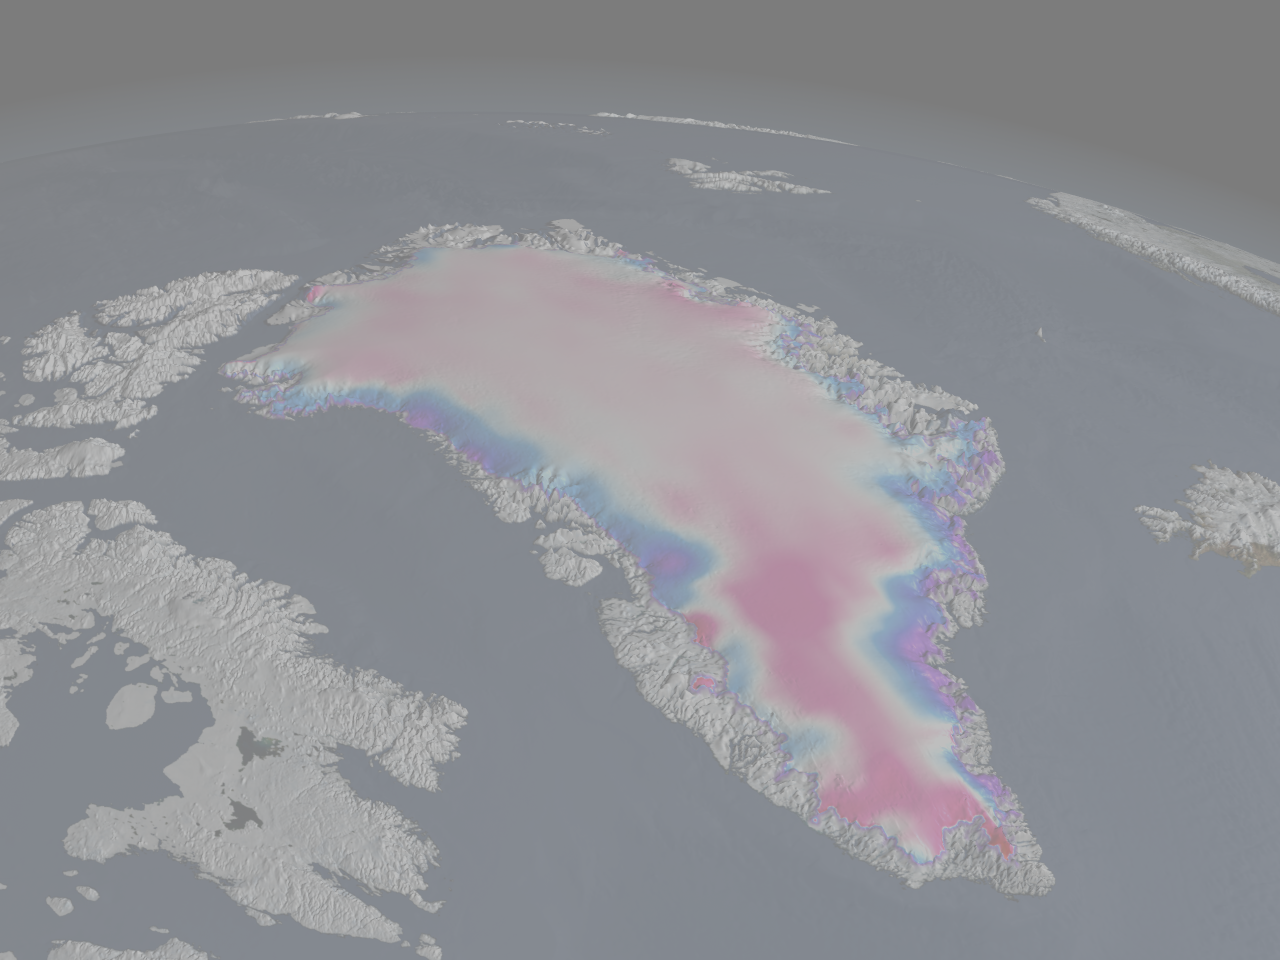
\includegraphics[width=\paperwidth]{Greenland_thinning_pale}}

\begin{frame}
  \titlepage
\end{frame}
}

\section[why Greenland?]{why compute Greenland's flow?}

\newcommand{\creditto}[1]{\footnotesize{\emph{#1}}}

\begin{frame}{Jakobshavn Isbr{\ae}, west Greenland}
 \begin{figure}
    \hspace{2cm}
 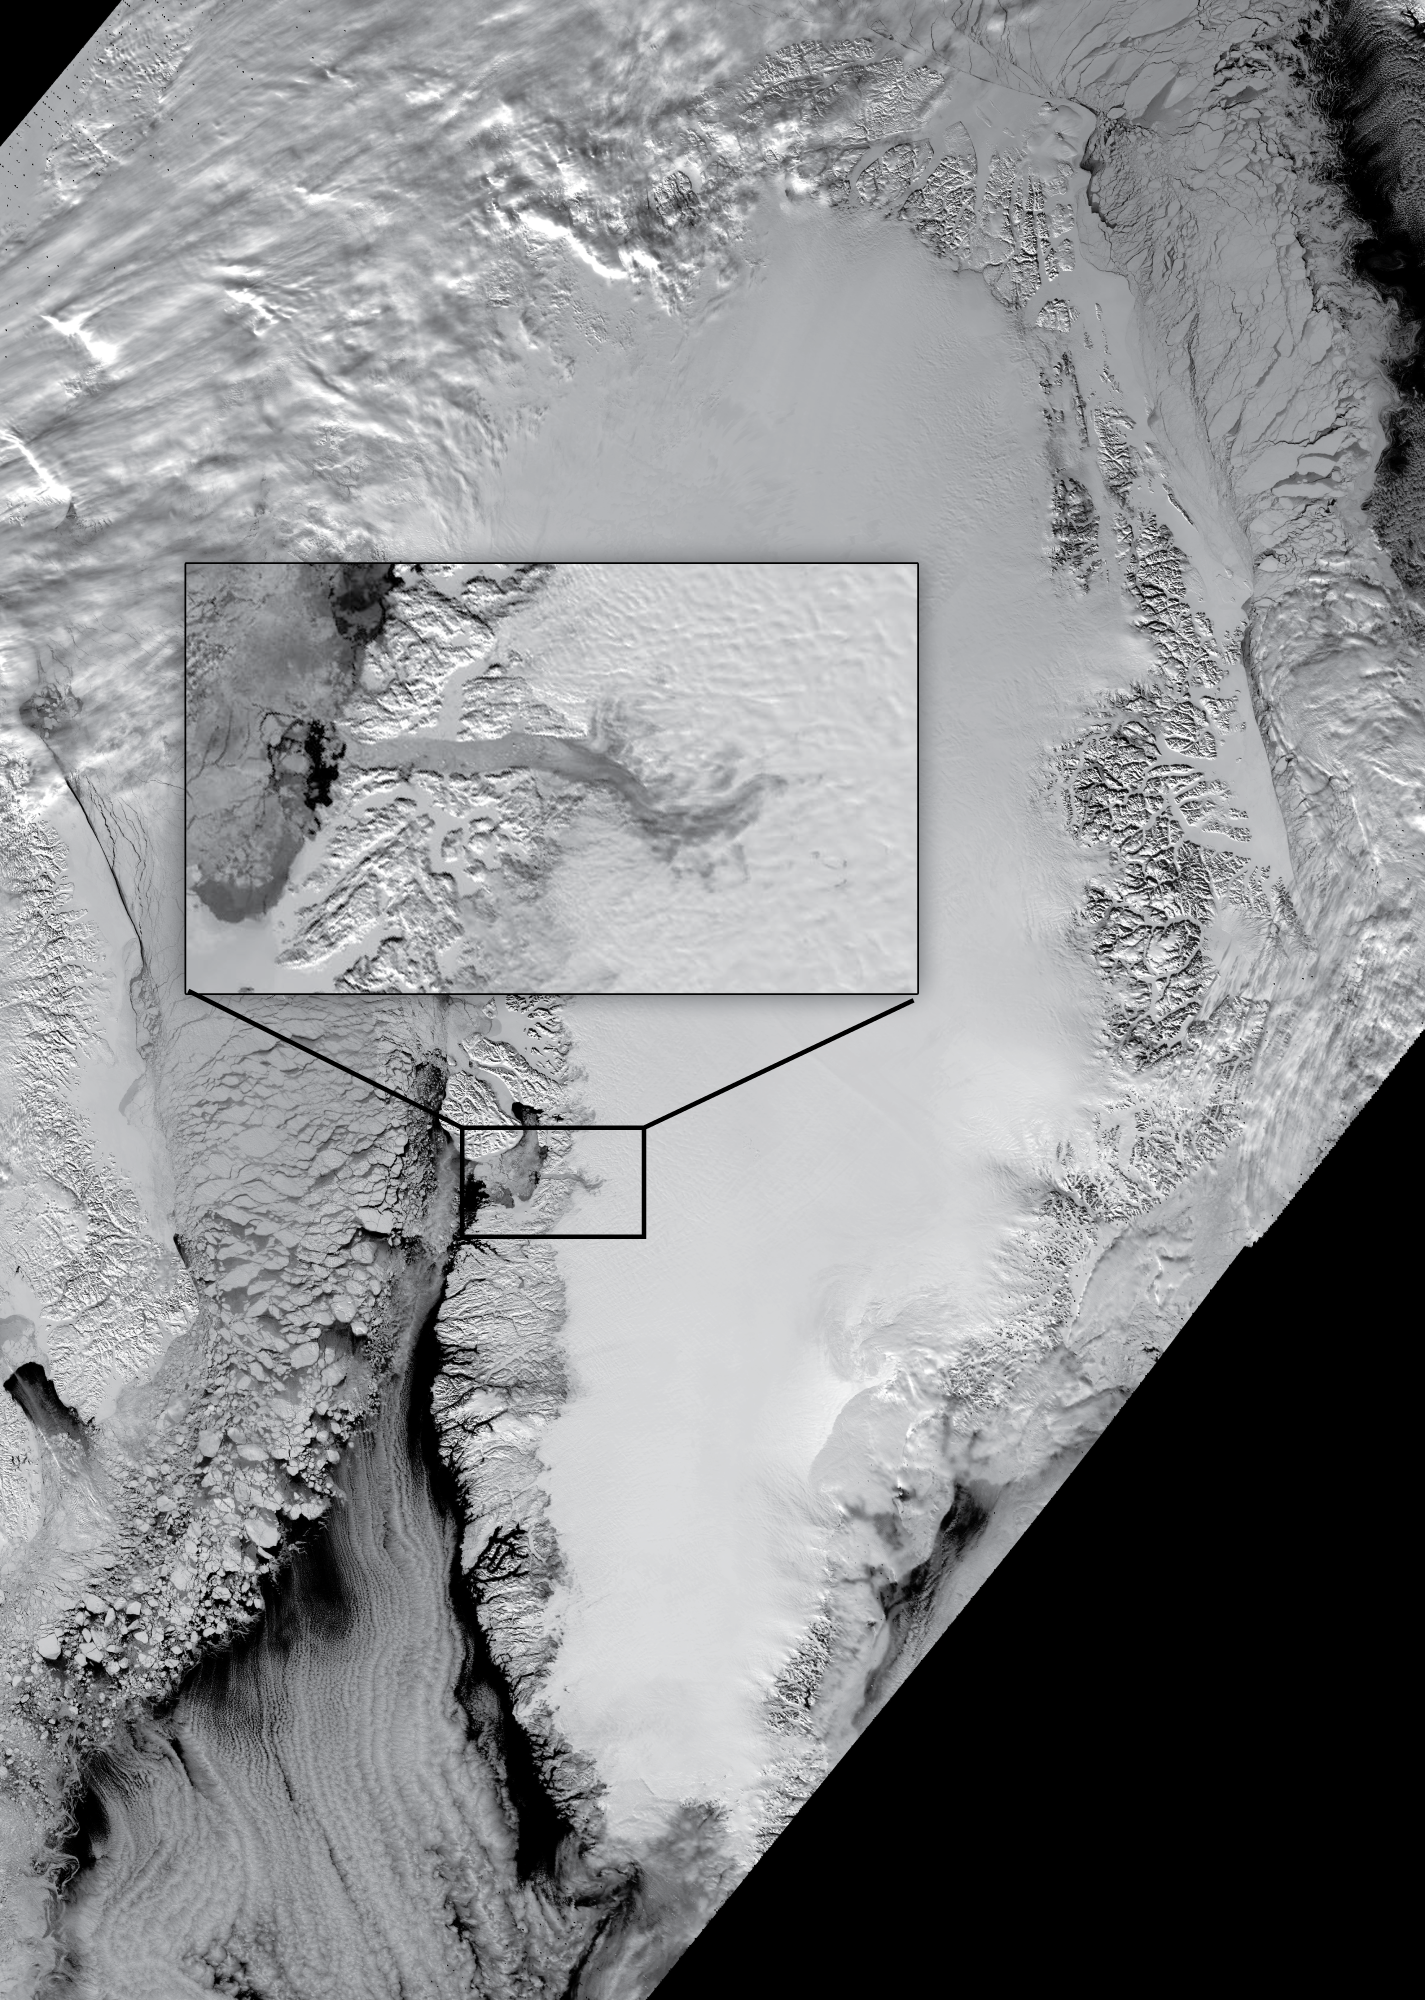
\includegraphics[height=0.85\textheight]{MODISGreenlandJakobshavn}  \quad  \creditto{\begin{minipage}[b]{3cm} MODIS image \\ M. Fahnestock\end{minipage}}
  \end{figure}
\end{frame}


\begin{frame}{Jakobshavn Isbr{\ae}, west Greenland}
 \begin{figure}
    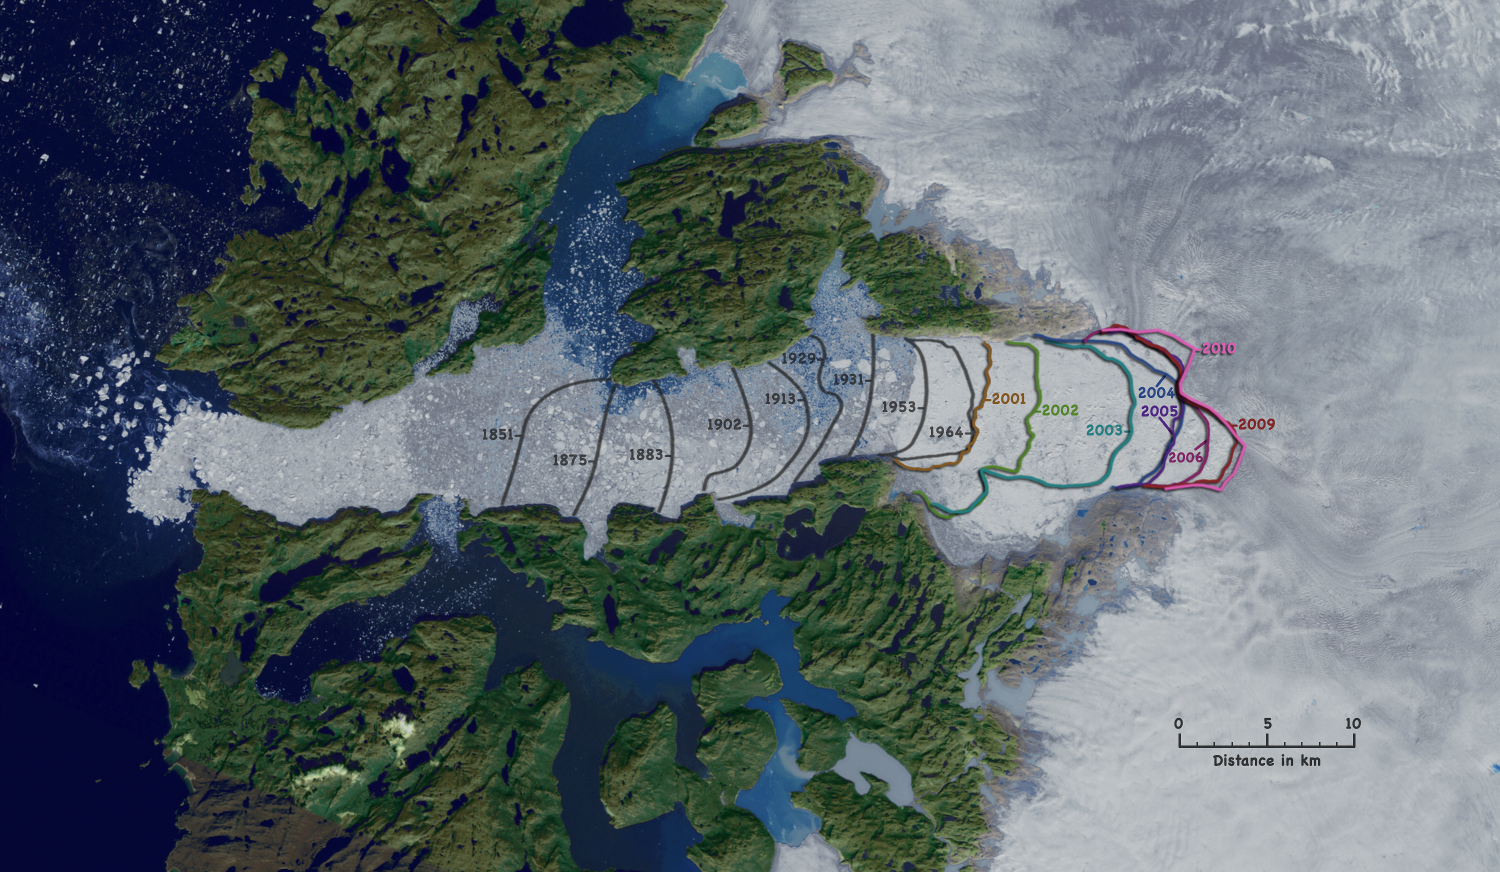
\includegraphics[width=\textwidth]{Jakobshavn_groundline_retreat} \\
    \creditto{NASA/Goddard Space Flight Center Scientific Visualization Studio}
  \end{figure}
\end{frame}


\begin{frame}{Speed-up of Jakobshavn Isbr{\ae}}
  \begin{itemize}
    \item almost doubled its flow speed between the 1992 and 2000:
      \begin{itemize}
      \item probably started by increase in ocean temperature from 1.7 C$^{\circ}$ in 1995 to 3.3 C$^{\circ}$ in 1998
      \item \dots thus increased melting under floating tongue
      \item loss of floating tongue and its ``backpressure'' on upstream grounded ice
      \item speed-up of grounded ice
      \end{itemize}
    \item now drains about 7\% of the entire ice sheet
  \end{itemize}
  \begin{figure}
    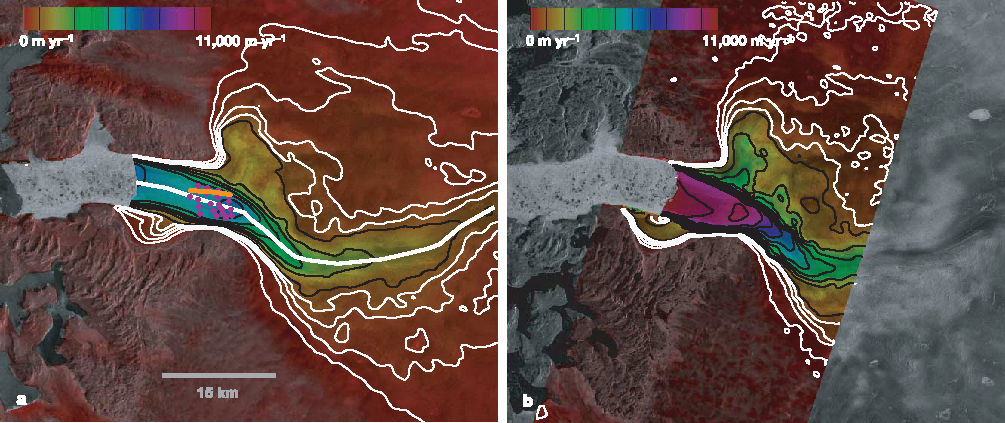
\includegraphics[width=0.8\textwidth]{Joughin2004Fig2} \\
    \creditto{Joughin et al. (2004)}
  \end{figure}
\end{frame}


\begin{frame}[label=ICESatElevation]{Elevation changes: surface melt and ``discharge''}
 \begin{figure}
   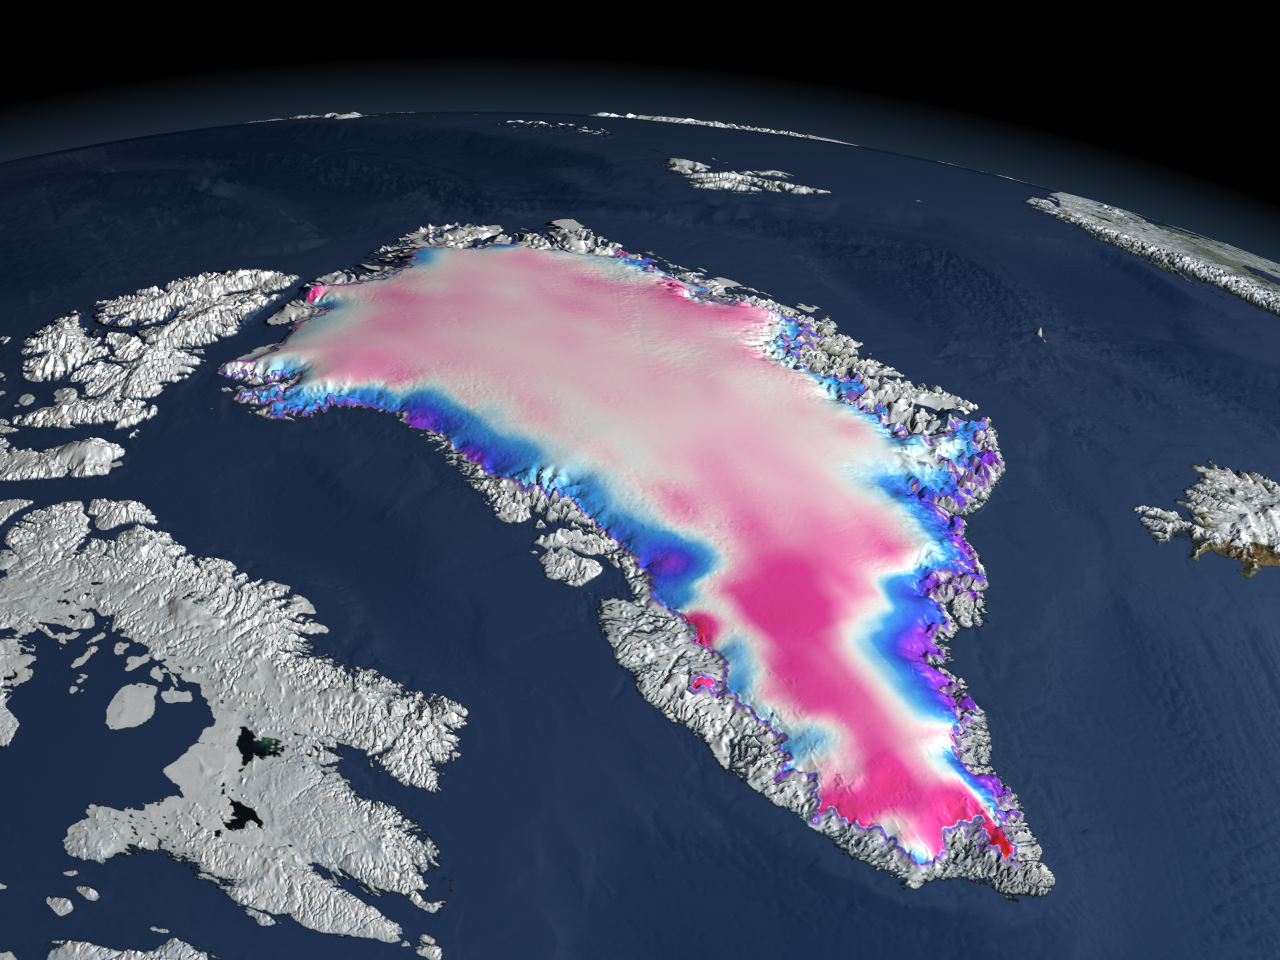
\includegraphics[height=7cm]{Greenland_thinning} \vspace{.1em}
   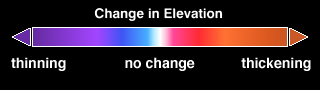
\includegraphics[height=1.25cm,angle=90]{ElevChangeColorBar} \\
    \creditto{IceSAT observations over 2003--2006 period; NASA/Goddard Space Flight Center Scientific Visualization Studio}
  \end{figure}
\end{frame}


\begin{frame}{The future of Greenland is the question}
  \begin{columns}[c]
    \begin{column}{.5\linewidth}
      \begin{itemize}
        \item before mid-90s mass loss was dominated by surface mass balance (= precipitation minus surface melt/runoff)
        \item since 2000, mass balance has been persistently negative
          \begin{itemize}
            \item decrease in surface mass balance (\alert{more melting beats more precipitation})
            \item increase in discharge (\alert{calving}) from ice flow
          \end{itemize}
        \item future mass loss partitioning: {\color{red}unknown}
        \item models need to predict which climate changes have which effects
      \end{itemize}
    \end{column}
    \begin{column}{.5\linewidth}
      \begin{figure}
        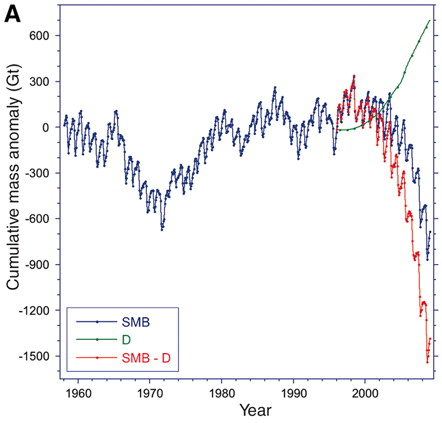
\includegraphics[width=\textwidth]{VanDenBroeke2009Fig2a} \\
        \creditto{van den Broeke et al. (2009)}
      \end{figure}
    \end{column}
  \end{columns}
\end{frame}


\setbeamertemplate{background canvas}
  {
     \tikz{\node[inner sep=0pt,opacity=1.0] {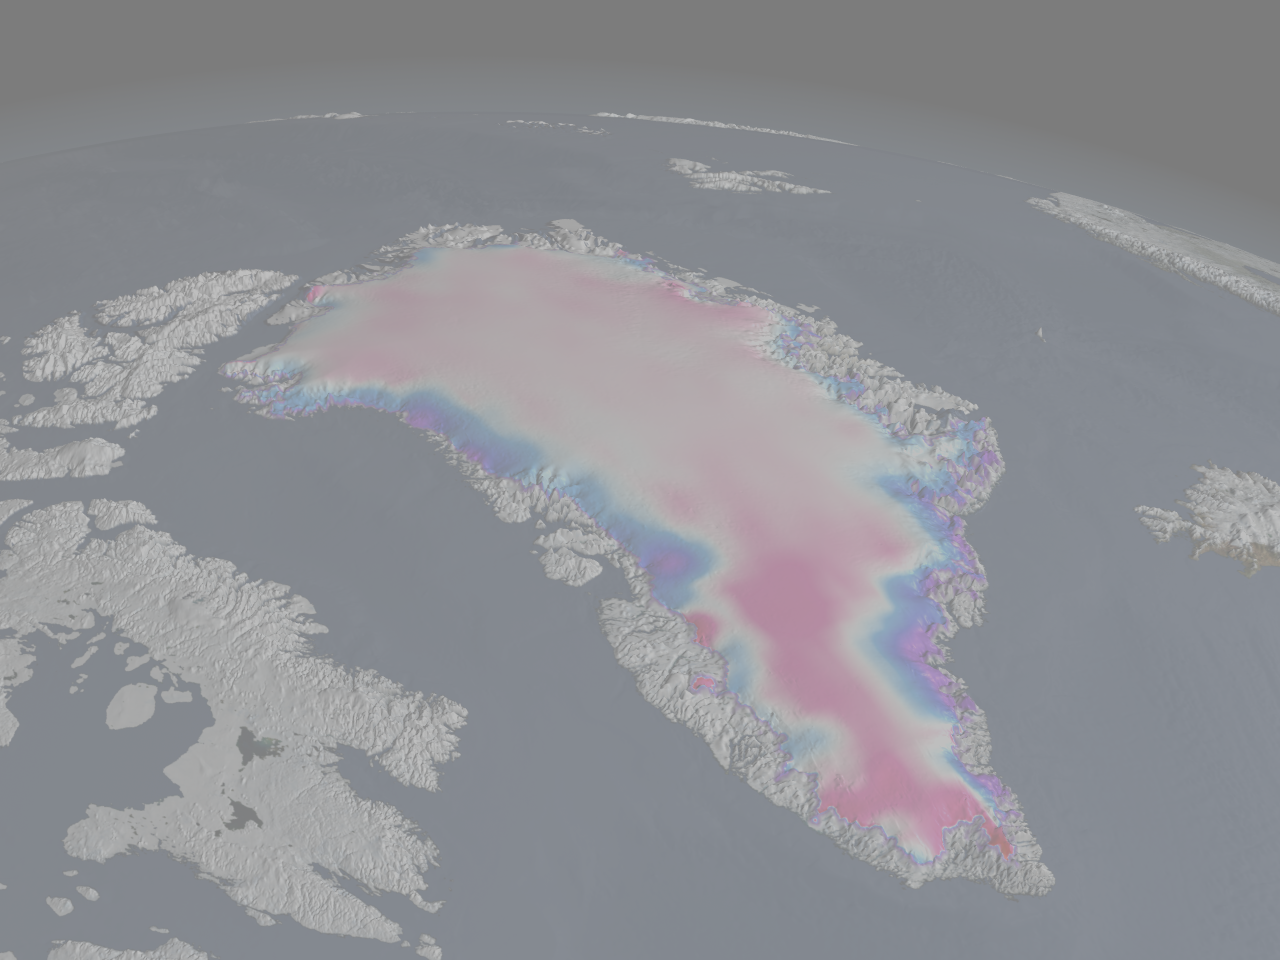
\includegraphics[height=
\paperheight,width=\paperwidth]{Greenland_thinning_pale}};}
} 

\begin{frame}
  \begin{transbox}
    \begin{block}{Why Greenland?}
      \begin{itemize}
      \item its changes affect future sea level rise
        \begin{itemize}
        \item 7\,m rise if completely melted \dots unlikely \dots is 1 or 2 m likely?
        \end{itemize}
      \item observations over the past decades show:
        \begin{itemize}
        \item rapid acceleration of outlet glaciers
        \item thinning around the margin
        \item increased mass loss
       \end{itemize}
      \item it's a testbed for ice sheet modeling:
        \begin{itemize}
        \item recent observational attention: lots of flights, ground measurements
        \item exhibits the kind of worrying dynamics we want to ``explain''
        \item Antarctic ice sheet has 10$\times$ the area thus 10$\times$ the cost
        \end{itemize}
      
      \end{itemize}
    \end{block}
  \end{transbox}
\end{frame}


\setbeamertemplate{background canvas}
{
%
} 


\section[modeling and observations]{ice sheets: modeling and observations}

\begin{frame}{How does an ice sheet lose mass?}
  \begin{figure}
    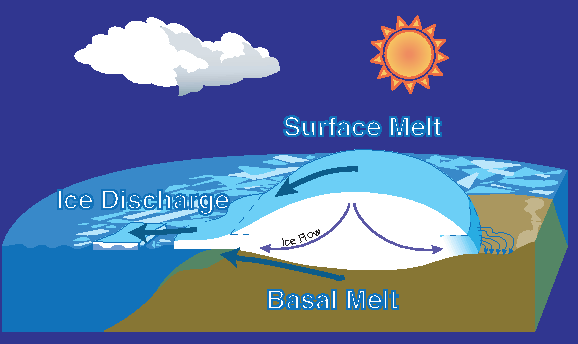
\includegraphics[width=\textwidth]{ice-sheet-cartoon}\\
    \creditto{modified from ICESat brochure}
  \end{figure}
\end{frame}


\begin{frame}{IPCC and ice sheet models}
  \begin{beamercolorbox}[rounded=true,shadow=true]{boxed}
    \begin{block}{IPCC (2007), Box 4.1: Ice Sheet Dynamics and Stability}
      ``\ldots but recent changes in ice sheet margins and ice streams cannot be simulated accurately with these models, \ldots.''
    \end{block}
  \end{beamercolorbox}
  \begin{itemize}
  \item $\text{IPCC} = \text{Intergovernmental Panel on Climate Change}$

\qquad \, $=\{\text{2007 Nobel Peace Prize winners}\} \setminus \{\text{Al Gore}\}$
  \item above statement $\Longrightarrow$ lots of attention from modelers
  \end{itemize}

  \begin{block}{progress report 2011:}

    \begin{itemize}
    \item PISM is doing a decent job reproducing the past two decades
      \begin{itemize}
      \item before anything else, get the present, observed period right!
      \item \alert{model validation}
      \end{itemize}
    \end{itemize}
  \end{block}
\end{frame}


\begin{frame}{Ice sheet model validation using}
 \begin{itemize}
  \item observed mean flow speed from 2000,2006--2008 (InSAR)
    \begin{figure}
      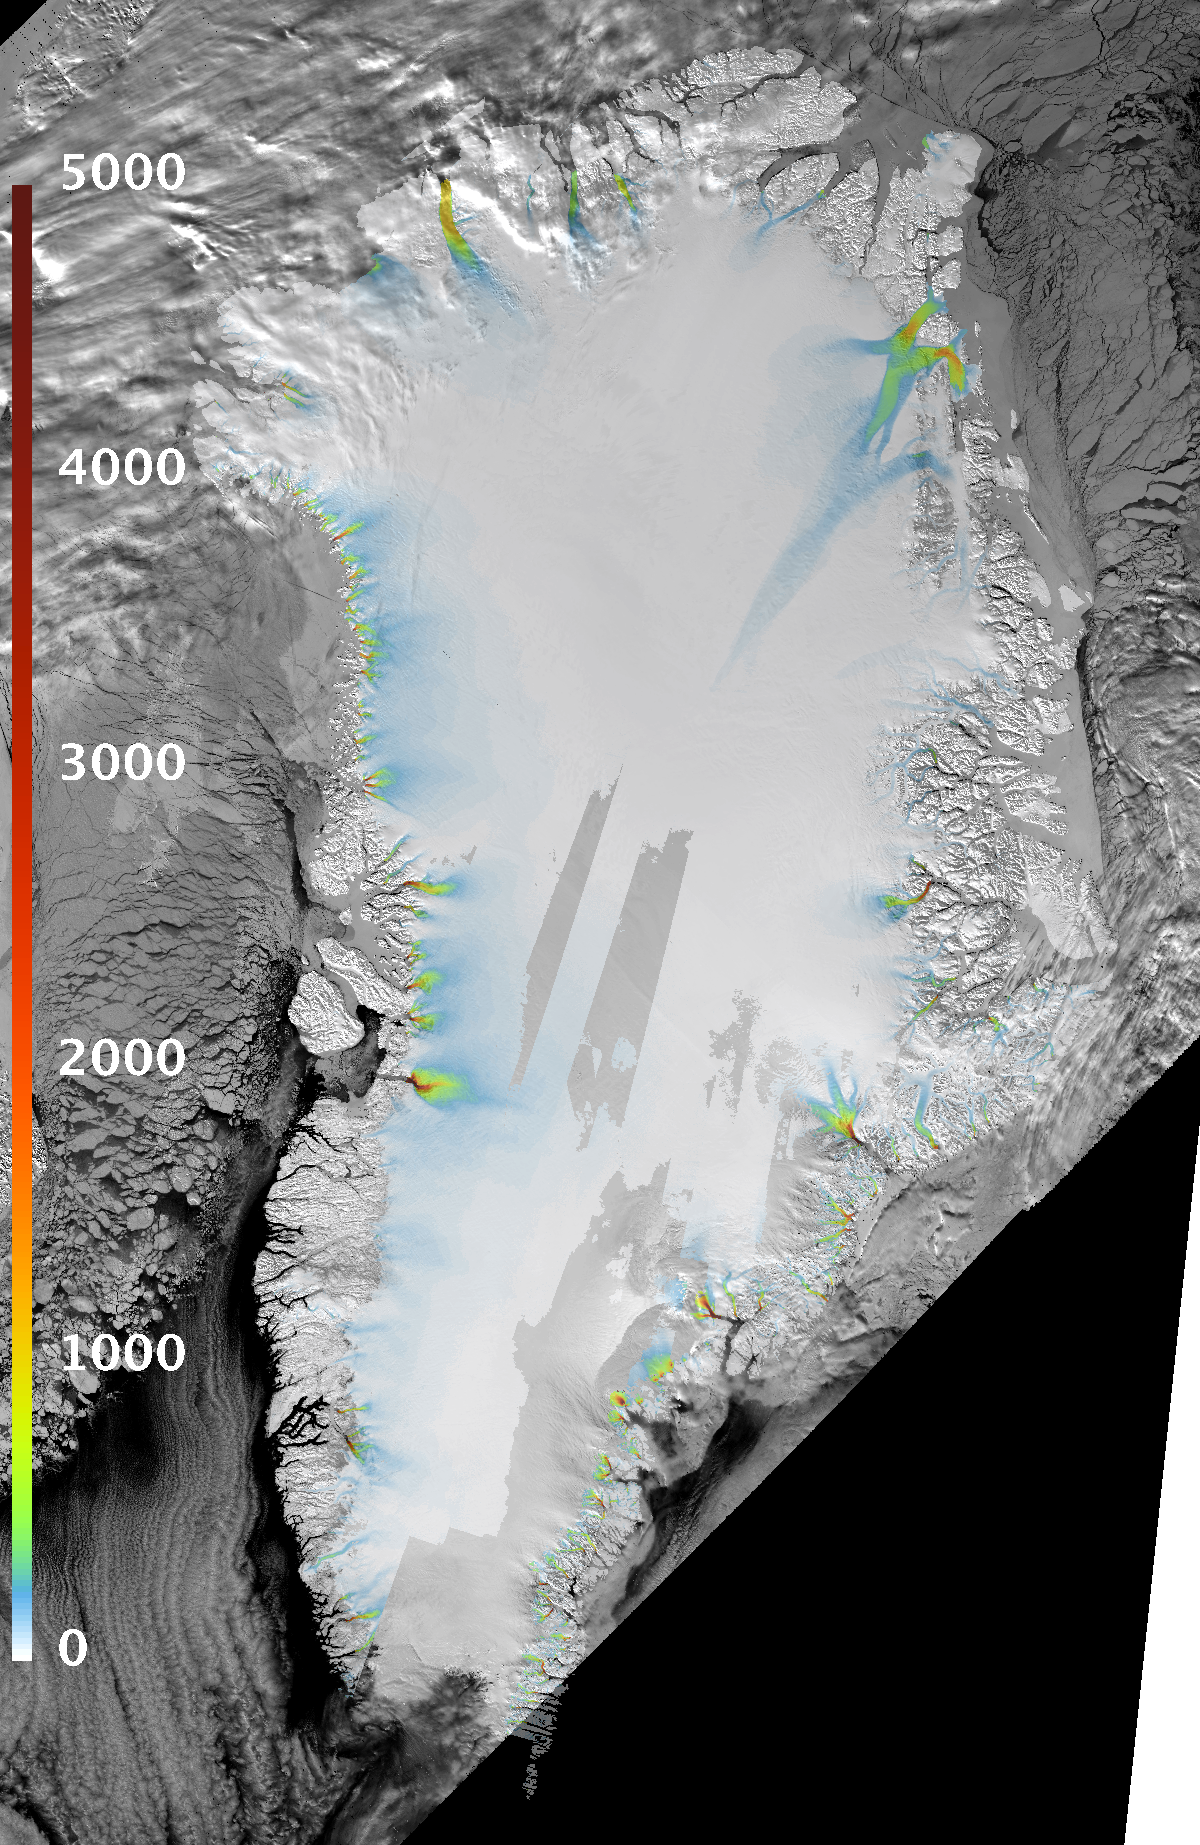
\includegraphics[height=3cm]{modis-insar}
    \end{figure}
  \item observed cumulative mass change from 2003--2009 (GRACE)
    \begin{figure}
      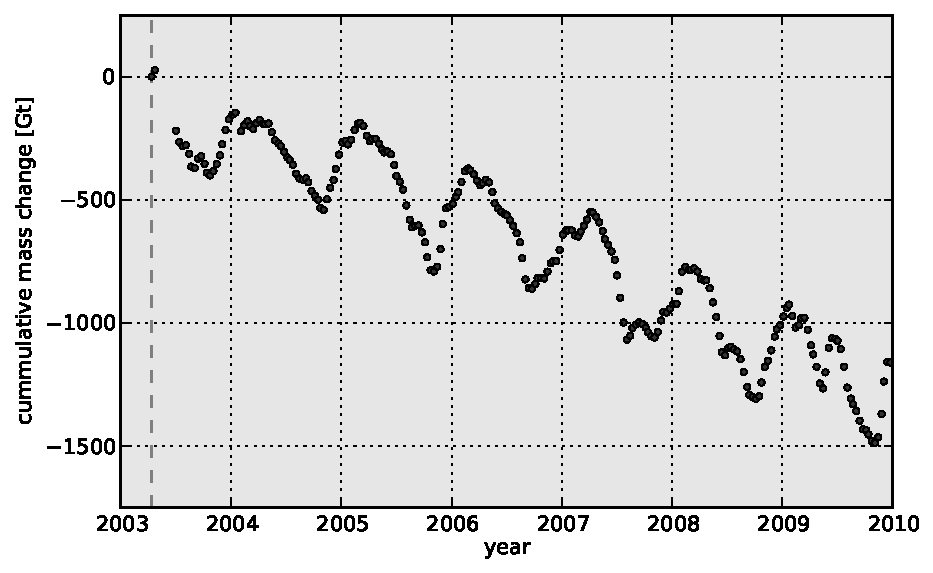
\includegraphics[height=3cm]{ts_grn_grace_2003-2010} 
    \end{figure}
  \end{itemize}
\end{frame}


\begin{frame}{Flow speed from InSAR}
  \begin{columns}[c]
    \begin{column}{.55\linewidth}
      \vspace{-.5cm}
      \begin{figure}
        \includegraphics<1>[width=0.9\textwidth]{insar_how_to}\\
        \creditto{credit: USGS}
      \end{figure}
    \end{column}
    \begin{column}{.5\linewidth}
      \vspace{-.5cm}
      \begin{figure}
        \includegraphics<1>[width=0.8\textwidth]{modis-insar}\\
        \creditto{credit: I. Joughin}
      \end{figure}
    \end{column}
  \end{columns}
\end{frame}


\begin{frame}
  \frametitle{Results: Jakobshavn Isbr{\ae}}
  \vspace{-2em}
  \begin{columns}[t]
    \begin{column}{.48\linewidth}
      \begin{figure}
        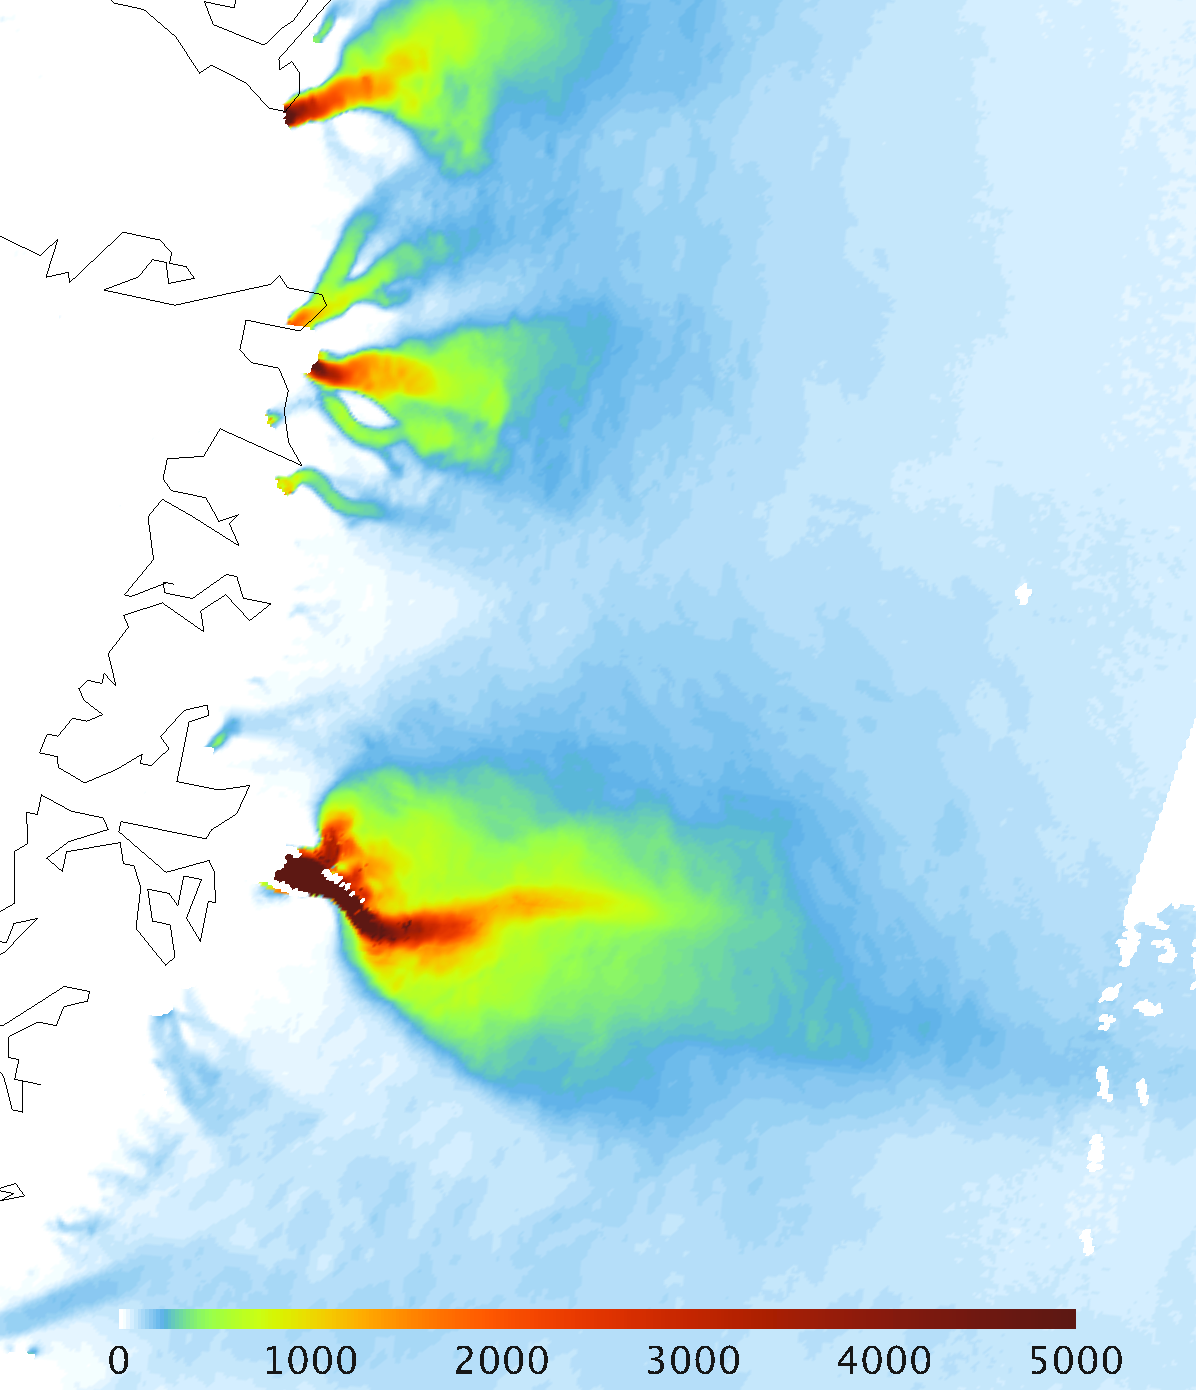
\includegraphics[width=\textwidth]{jak-insar-csurf} \\
        \small{InSAR (\creditto{Joughin et al., 2010})}
      \end{figure}
    \end{column}
    \begin{column}{.48\linewidth}
      \begin{figure}
        \includegraphics<1>[width=\textwidth]{jak5km-ssa-csurf} \\
        \small{PISM: 5\,km grid resolution}
      \end{figure}
    \end{column}
  \end{columns}
\end{frame}


\begin{frame}
  \frametitle{Results: Jakobshavn Isbr{\ae}}
  \vspace{-2em}
  \begin{columns}[t]
    \begin{column}{.48\linewidth}
      \begin{figure}
        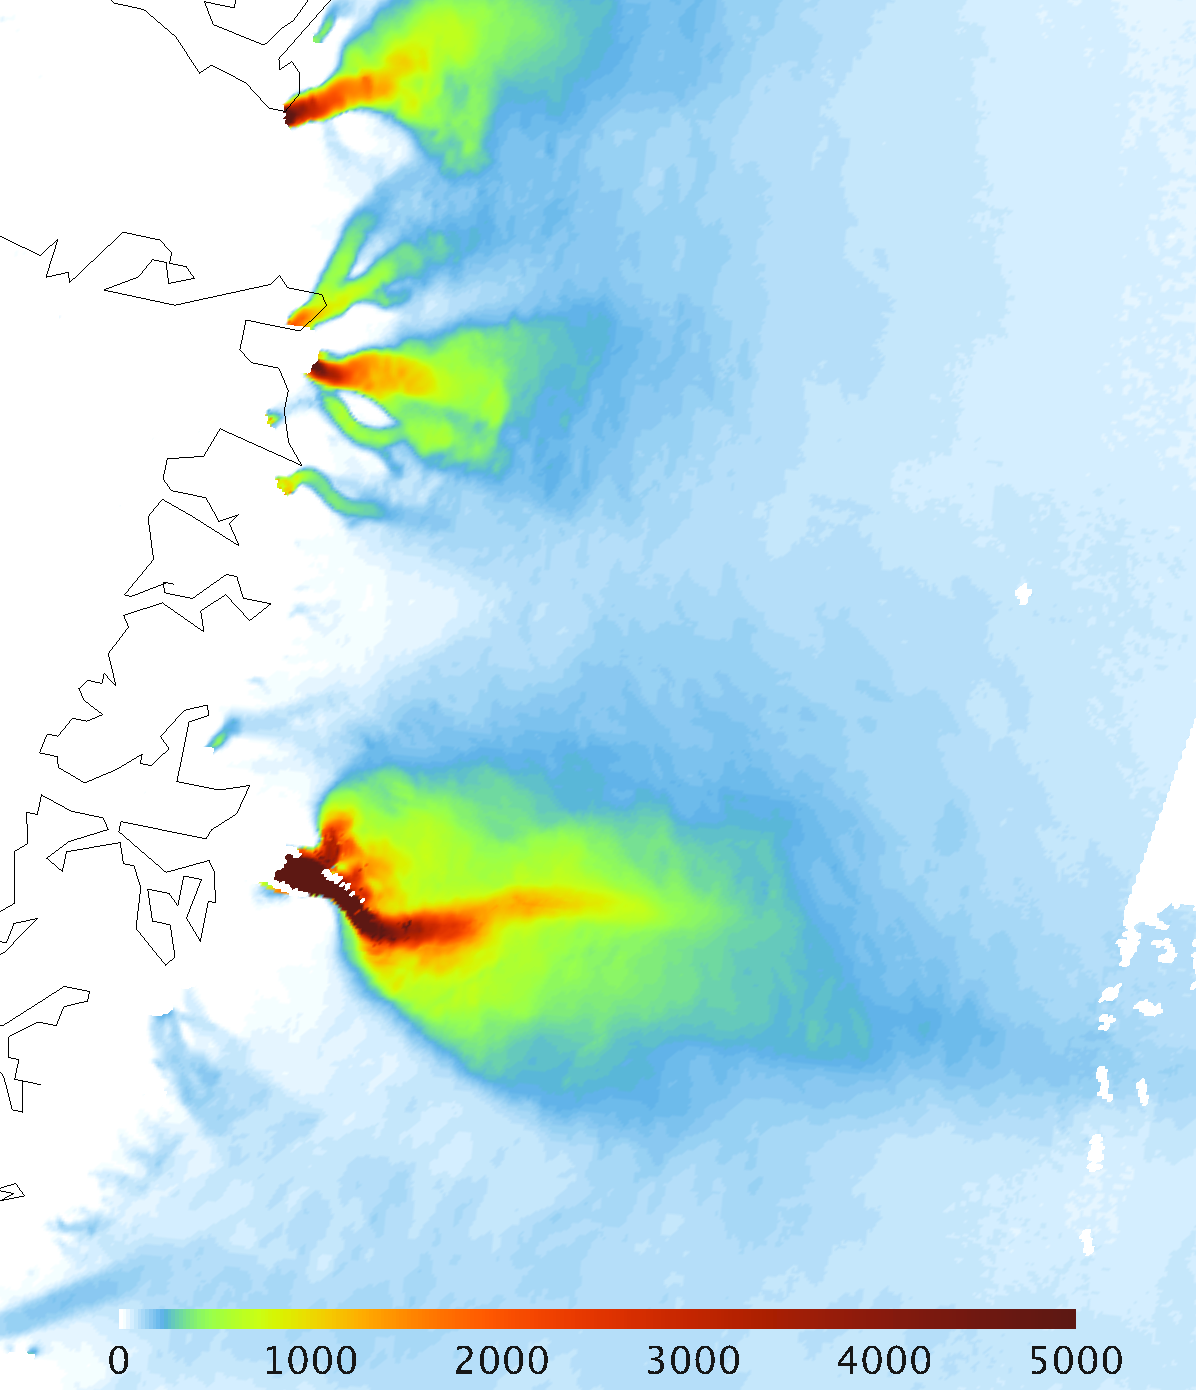
\includegraphics[width=\textwidth]{jak-insar-csurf} \\
        \small{InSAR (\creditto{Joughin et al., 2010})}
      \end{figure}
    \end{column}
    \begin{column}{.48\linewidth}
      \begin{figure}
        \includegraphics<1>[width=\textwidth]{jak2km-ssa-csurf} \\
        \small{PISM: 2\,km grid resolution}
      \end{figure}
    \end{column}
  \end{columns}
\end{frame}


\begin{frame}
  \frametitle{Results: Jakobshavn Isbr{\ae}}
  \vspace{-2em}
  \begin{columns}[t]
    \begin{column}{.48\linewidth}
      \begin{figure}
        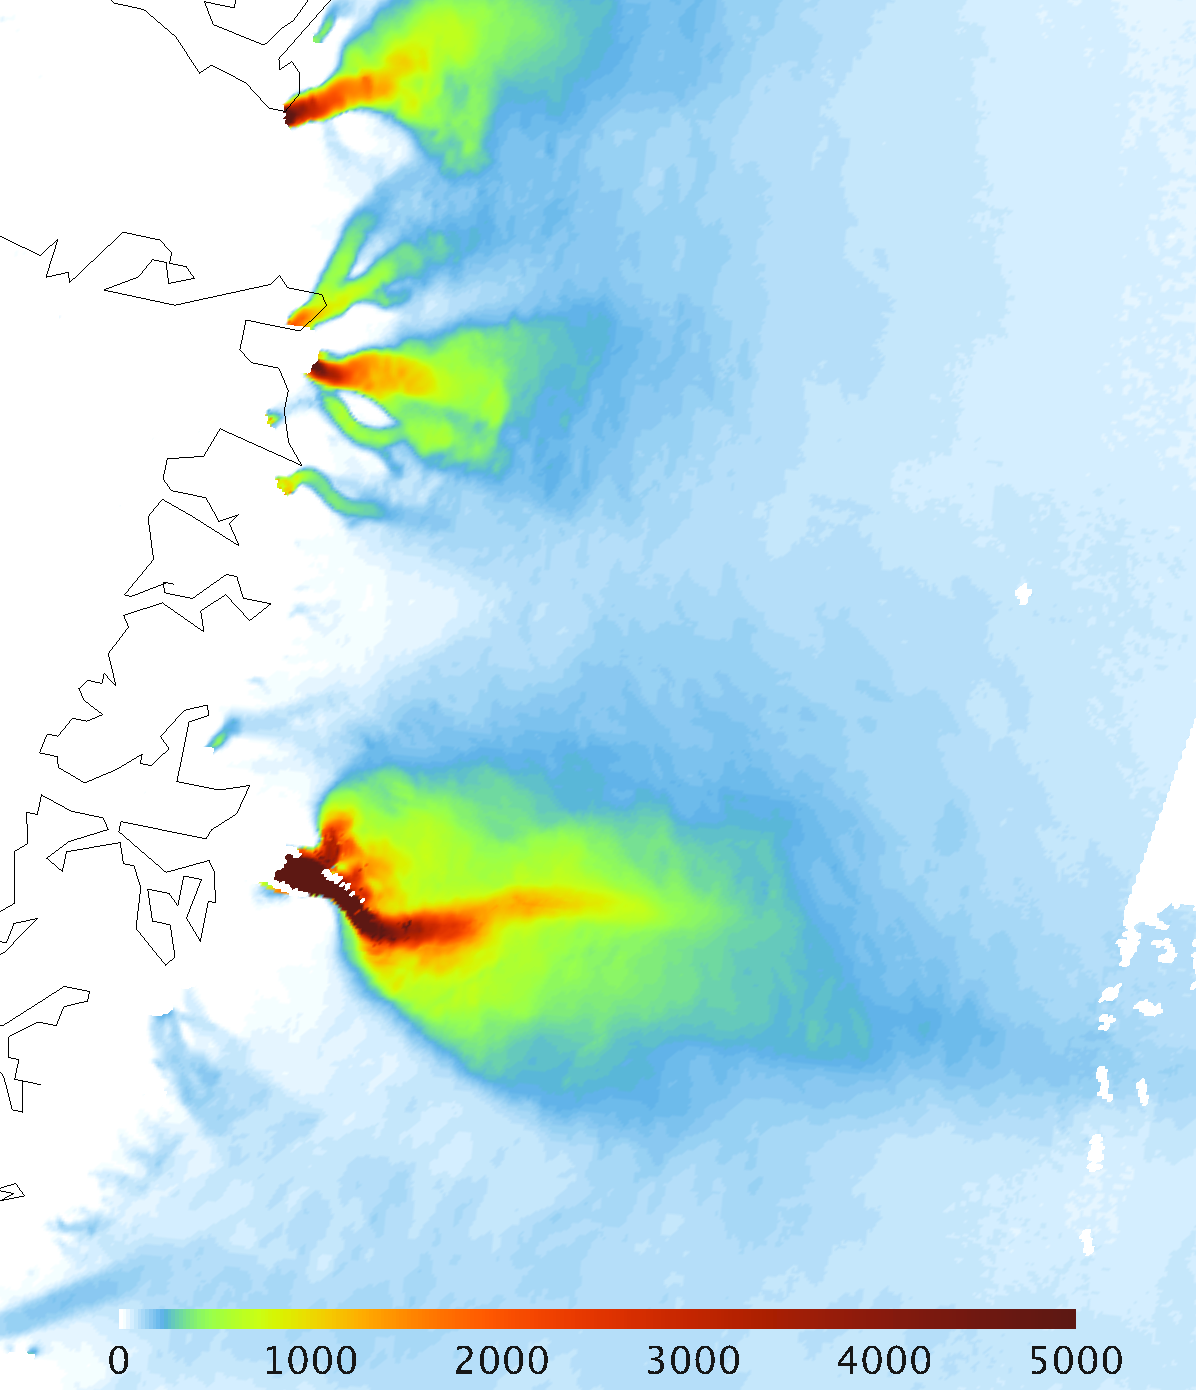
\includegraphics[width=\textwidth]{jak-insar-csurf} \\
        \small{InSAR (\creditto{Joughin et al., 2010})}
      \end{figure}
    \end{column}
    \begin{column}{.48\linewidth}
      \begin{figure}
        \includegraphics<1>[width=\textwidth]{jak1km-ssa-csurf} \\
        \small{PISM: 1\,km grid resolution}
      \end{figure}
    \end{column}
  \end{columns}
\end{frame}


\begin{frame}
  \frametitle{Gravity Recovery and Climate Experiment (GRACE)}
    \begin{figure}
       \includegraphics<1>[height=3.75cm]{grace-satellites} \hspace{2em}
       \includegraphics<1>[height=3.75cm]{grace-trend} \\
       \footnotesize{\emph{thanks to A.~Arendt}}
     \end{figure}
  \begin{itemize}
  \item precisely measures distance between pair of satellites
  \item estimates deviation of gravity field from uniform sphere shape
  \end{itemize}
\end{frame}


\begin{frame}
  \frametitle{Observed mass changes}
  % as in previous animation, but updated until 2010
    \begin{figure}
      \includegraphics<1>[width=.85\textwidth]{ts_grn_grace_2003-2010}
      \includegraphics<2>[width=.85\textwidth]{ts_grn_grace_trend_2003-2010}\\
      \footnotesize{Luthcke, et al.~(unpublished; new high-resolution solutions)}
   \end{figure}
\end{frame}


\begin{frame}{Modeled and observed mass changes}
  \begin{figure}
    \includegraphics<1>[width=.7\textwidth]{ts_grn_mass_2003-2010}
    \includegraphics<2>[width=.7\textwidth]{ts_grn_mass_2003-2010_CONST1}
  \end{figure}
  \begin{itemize}
  \item new coupled models of Greenland
    \begin{itemize}
    \item PISM $+$ regional climate model (HIRHAM at DMI Copenhagen)
    \end{itemize}
  \end{itemize}
\end{frame}


\begin{frame}{What is PISM?}

\begin{itemize}
\item PISM = Parallel Ice Sheet Model \qquad \texttt{www.pism-docs.org}
\item open source (C++, python), PETSc-over-MPI, regular grid
\item adaptive time-stepping
\item supported by NASA; now a joint project with PIK in Germany
\item<1-> the best ice sheet model in the world
\item<2> \dots was developed in Fairbanks
\end{itemize}

\begin{center}
    user base: \quad %FIXME: 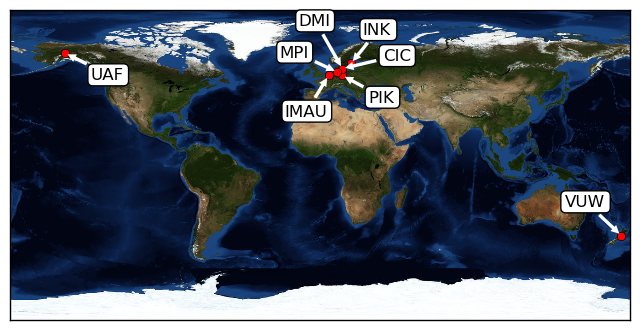
\includegraphics[width=0.6\textwidth]{pism-user-world}
\end{center}
\end{frame}


\section[scaling-up]{scaling-up: how to get more ISM from HPC}

\begin{frame}{Scaling}
\begin{itemize}
\item plan for the rest of my talk: beat up PISM because it scales badly
\item \dots though it scales \emph{way} better than any other current ISM
\item definitions in convenient 2D grid case:
  \begin{itemize}
  \item \alert{strong scaling}: for fixed problem, 
  
  \centerline{4$\times$ the number of processors $\implies$ (1/4)th the execution time}
    \begin{center}
    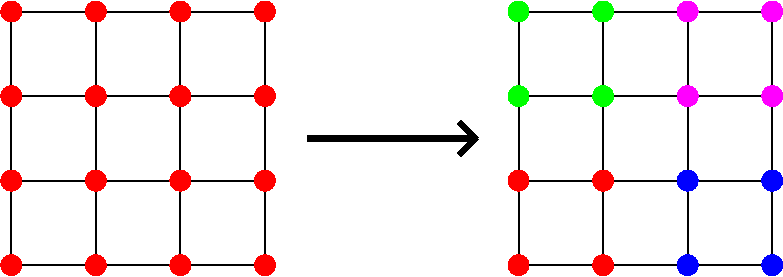
\includegraphics[height=1.8cm]{stronggrid}
    \end{center}
  \item \alert{weak scaling}: for fixed number of d.o.f.s \emph{per processor},
  
  \centerline{4$\times$ the number of processors $\implies$ \emph{same} execution time}
    \begin{center}
    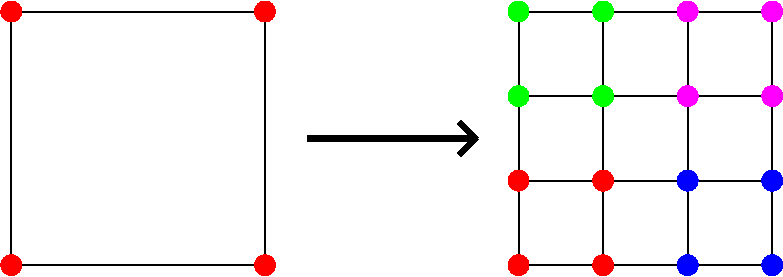
\includegraphics[height=1.8cm]{weakgrid}
    \end{center}
  \end{itemize}
\end{itemize}
\end{frame}


\begin{frame}{Min prerequisite for weak scaling: convergence}
\begin{columns}
\begin{column}{0.45\textwidth}
  \begin{itemize}\small
  \item six runs, each 100 model year with same data
  \item on refining grids: 40, 20, 10, 5, 2.5 km
  \item surface velocity (m/year) $\to$
  \item my first informal study
  \item results:
    \begin{tabular}{lcr}
    res & procs & wall clock \\ \hline
    40 km & 1 & 8 sec \\
    \color{red} 20 km & \color{red} 1 & \color{red} 75 sec \\
    \color{red} 10 km & \color{red} 64 & \color{red} 57 sec \\
    5 km & 64 & 14 min \\
    3 km & 128 & 56 min \\
    2 km & 128 & 285 min
    \end{tabular}
  \item on Cray XT5
    \begin{itemize}
    \item \texttt{pingo.arsc.edu}
    \end{itemize}
  \end{itemize}
  \normalsize
\end{column}
\begin{column}{0.55\textwidth}
  \vspace{-1cm}
  \begin{center}
  \animategraphics[autoplay,loop,height=8cm]{1.0}{anim/g_csurf_frames_}{0}{5} 
  \end{center}
\end{column}
\end{columns}
\end{frame}


\begin{frame}{Weak scaling: the reality}
\begin{columns}
\begin{column}{0.4\textwidth}
  \begin{itemize}
  \item here's the problem $\to$
    \begin{itemize}
    \item 100 model year runs
    \item increase d.o.f.s and processors in proportion
      \begin{itemize}
      \item a la weak scaling
      \end{itemize}
    \item it is \alert{not} giving constant-time for whole run
    \item<2-> it is giving constant-time per model time step
      \begin{itemize}
      \item but who cares
      \end{itemize}
    \end{itemize}
  \item<3> we observe: \alert{short time steps on fine grids blocks weak scaling}
  \end{itemize}
\end{column}
\begin{column}{0.6\textwidth}
        \includegraphics<1>[width=\textwidth]{weak-time}
        \includegraphics<2>[width=\textwidth]{weak-time-per-step}
        \includegraphics<3>[width=\textwidth]{dt-dx-power}
\end{column}
\end{columns}
\end{frame}


\begin{frame}{Weak scaling: the troubles}
  \begin{enumerate}
  \item[1] PISM evolves temperature and geometry by \alert{explicit} time-stepping
    \begin{itemize}
    \item major evolution equation is wildly-nonlinear diffusion
    \item ice thickness $H$ changes by
    	$$\frac{\partial H}{\partial t} \stackrel{\ast}{=} \nabla \cdot \left(C H^5 |\nabla H|^2 \nabla H\right)$$
    \item explicit method scales badly because
        $$\Delta t \sim \Delta x^2$$
    \item \emph{implicit time steps, you idiot!}
    \item but we are not solving PDEs; boundary value problem is $\ast$ subject to inequality
    	$$H\ge 0$$
    \item so we don't really know how to solve well-posed implicit time steps
    \end{itemize}
  \end{enumerate}
\end{frame}


\begin{frame}{Scaling: results so far; idealized ice sheets}
  \vspace{-0.5cm}
  \begin{figure}
    \includegraphics<1>[height=.6\textheight]{timing_P1_low}
    \includegraphics<2>[height=.6\textheight]{BrownSmithAhmadia_weak_fig.png}
  \end{figure}
  
  \vspace{-0.5cm}
  \begin{itemize}
  \item<1> PISM: strong scaling on time-dependent run including many 2D stress solutions
  \item<2> Jed Brown's hydrostatic ice solver [\emph{submitted 2011}]: awesome weak scaling on time-independent 3D stress solver; \emph{not yet in PISM!}
  \end{itemize}
\end{frame}


\begin{frame}{Weak scaling: the troubles}
\begin{columns}
\begin{column}{0.5\textwidth}
  \begin{enumerate}
  \item[2] \alert{liquid water} at boundaries
    \begin{itemize}
    \item big lakes form and drain \dots in 90 minutes  (upper)
    \item hydrograph shows brief summer period of surface melt (lower)
    \item ice flow model must ``see'' liquid runoff at surface \emph{and} its effect on subglacial resistance
      \begin{itemize}
      \item boundary liquid timescales are minutes--weeks
      \item ice sheet model runs are decades--millenia
      \end{itemize}
    \end{itemize}
  \end{enumerate}
\end{column}
\begin{column}{0.5\textwidth}
\vspace{-1cm}

      \begin{center}
        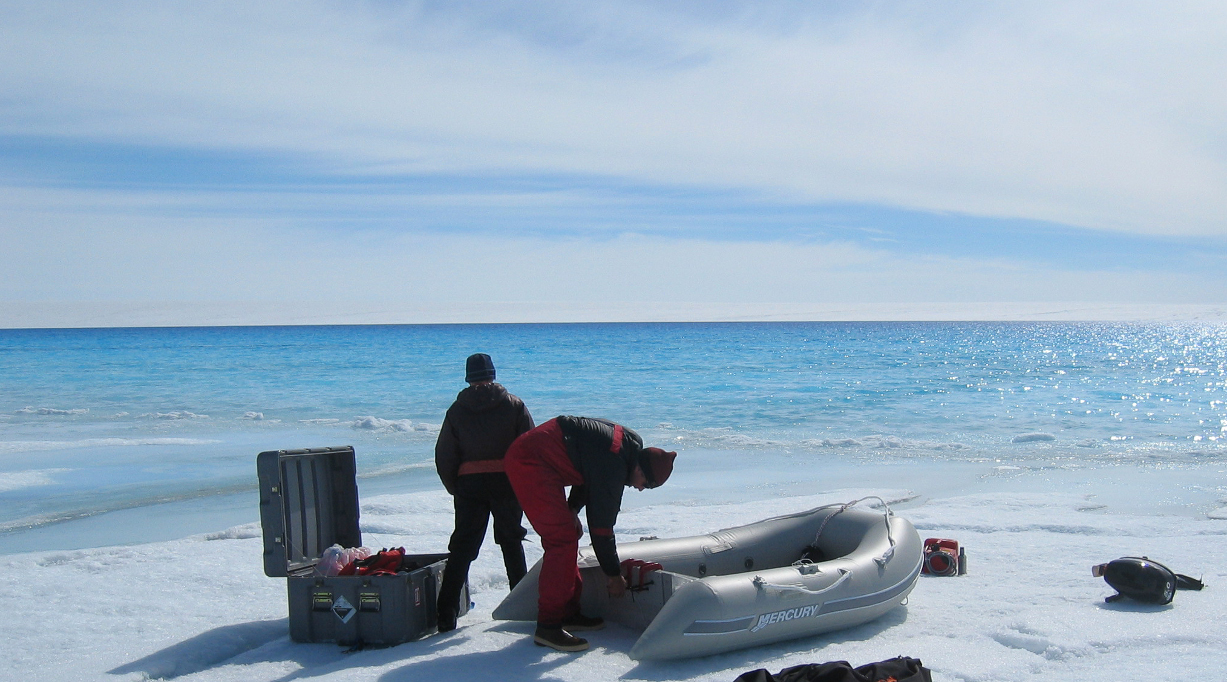
\includegraphics[width=\textwidth]{Greenland06-10}
        
        \creditto{S.~Das}
      \end{center}

      \begin{center}
        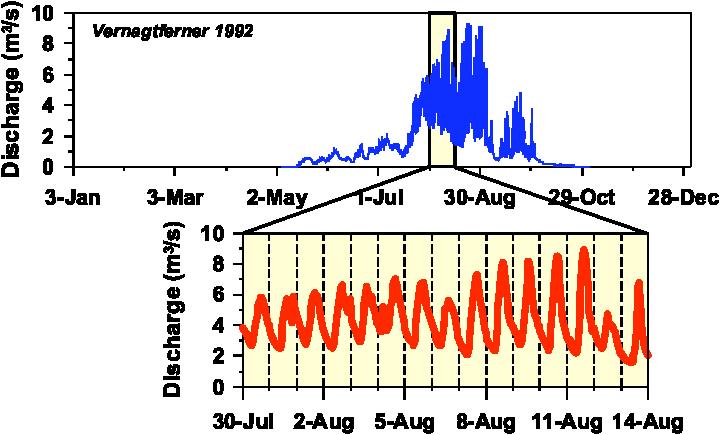
\includegraphics[width=0.9\textwidth]{ferner}
        
        \creditto{R.~Hock et al.~(2005)}
      \end{center}
\end{column}
\end{columns}
\end{frame}


\begin{frame}{Weak scaling: the troubles}
\begin{columns}
\begin{column}{0.45\textwidth}
  \begin{enumerate}
  \item[3] solve PDEs on domain with fractal boundary
    \begin{itemize}
    \item velocity is big near the boundary
    \item boundary is a \alert{coastline} \dots Mandelbrot warned us about those things
    \item at each timestep, want to solve nonlinear elliptic problems on this fractal
    \end{itemize}
  \end{enumerate}
\end{column}
\begin{column}{0.55\textwidth}
\vspace{-1cm}
      \begin{center}
        \includegraphics[width=\textwidth]{anim/g_csurf_frames_5.png}
      \end{center}
\end{column}
\end{columns}
\end{frame}


\section*{}

\setbeamertemplate{background canvas}
  {
     \tikz{\node[inner sep=0pt,opacity=0.4] {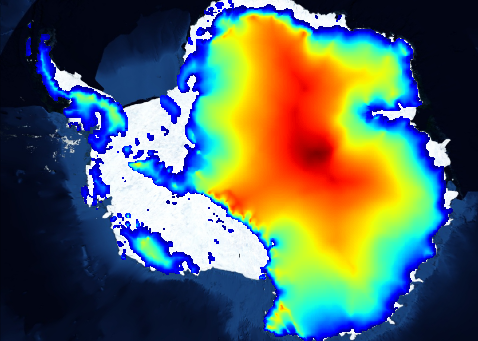
\includegraphics[height=\paperheight]{a10km_hybrid_0_usurf}};}
} 

\begin{frame}
\begin{transbox}
\begin{block}{Summary}
  \begin{itemize}
  \item model Greenland ice sheet flow! it is on the move!
  \item PISM is getting good fit to observed flow speeds, mass changes
  \item challenges to scaling:
    \begin{itemize}
    \item equations need new thinking
      \begin{itemize}
      \item[$\circ$] need well-posed implicit time steps
      \item[$\circ$] and better solvers too
      \end{itemize}
    \item short time-scale processes on all ice sheet surfaces
      \begin{itemize}
      \item[$\circ$] liquid water
      \end{itemize}
    \item fast ice dynamics along fractal boundaries
    \end{itemize}
  \item much bigger Antarctic ice sheet in the background
  \item \alert{thanks for your attention!}
  \end{itemize}
\end{block}
\end{transbox}
\end{frame}

\setbeamertemplate{background canvas}
{
%
}

\end{document}
